\documentclass[14pt, bachelor, substylefile=bachelor.rtx]{disser}%twoside, 

\usepackage[a4paper, includefoot, left=3cm, right=1cm, top=2cm, bottom=2cm, headsep=1cm, footskip=1cm]{geometry}

\pagestyle{footcenter}
\chapterpagestyle{footcenter}

\usepackage[T2A]{fontenc}
\usepackage[utf8x]{inputenc}
\usepackage[english, russian]{babel}
\ifpdf\usepackage{epstopdf}\fi
\setcounter{tocdepth}{2}

\usepackage{comment}
\usepackage{amssymb}

% вставлять используемые пакеты сюда
% hyperref должен быть самым последним, иначе будут  баги с \chapter \section и \subsection

\usepackage[
pdfstartview   = FitH,
bookmarksopen  = true,bookmarksopenlevel=0,
plainpages     = false,pdfpagelabels,
pagebackref    = true,
pdftoolbar     = false,
unicode,
pdftex,
hidelinks
]{hyperref}

\renewcommand{\leq}{\leqslant}


\begin{document}
    \institution{%
        Министерство образования и науки Российской Федерации \\
        Федеральное агентство по образованию \\
        Федеральное государственное автономное образовательное учреждение\\ высшего образования «Национальный исследовательский университет \\«Московский институт электронной техники»\\
        Факультет МПиТК\\
        Кафедра ВМ-1
    }
\title{ВЫПУСКНАЯ КВАЛИФИКАЦИОННАЯ РАБОТА}
%\title{ДИССЕРТАЦИЯ\\[-14pt]на соискание ученой степени\\МАГИСТРА}
%\topic{\normalfont\scshape %
%    FIXME <<Название>>}
\topic{\normalfont\scshape<<Оценка линейного искажающего оператора в задаче восстановления изображения>>}

\coursenum{01.04.04}
\course{Прикладная математика}
%\masterprog{Математические методы и моделирование\\ \>\ \ в естественнонаучной и технической сферах}
\author{Терентьев И.~В.}
\group{ВМ-40}

%\apname{Прокофьев А.А.}

\sa {Умняшкин С.~В.}
\sastatus{профессор, д.ф.-м.н.}
\city{Москва}
\date{2018}

\maketitle

\tableofcontents

\intro

Льем воду.

Так как нужно 60-80 страниц.

А это нелегко без нее.

\chapter{Обзор проблематики восстановления изображений}
\section{Модель искажения}\label{seqtion:distortionModel}
Изображение~--- это двумерная проекция трёхмерной сцены. Записывающая система(камера) проецирует сцену на двумерную область~--- изображение. Под изображением понимаем двумерный дискретный сигнал $f(x,y)$, где $0\leq x \leq M$, $0\leq y\leq N$ ($M$, $N$~--- ширина и высота изображения соответственно). В данной работе рассматриваем только обработку полутоновых изображений со значениями яркости $0\leq f(x,y)\leq 1$.

\begin{figure}[h!]
	\tikzset{%
		block/.style    = {draw, thick, rectangle, minimum height = 3em,
			minimum width = 3em, node distance = 3cm},
		sum/.style      = {draw, circle, node distance = 3cm}, % Adder
		input/.style    = {coordinate}, % Input
		output/.style   = {coordinate, node distance = 3cm} % Output
	}
    \centering
    \begin{tikzpicture}[auto, thick, node distance=2cm, >=triangle 45]
    \draw
        node [input, name=in] {} 
        node [block, right of=in] (hxy) {$h(x,y)$}
        node [sum, right of=hxy] (sum1) {\Large$+$}
        node [input, above of=sum1] (noize) {}
        node [output, right of=sum1] (out){$g(x,y)$};
    \draw[->](in)     -- node {$f(x,y)$}(hxy);
    \draw[->](hxy)    -- node {$s(x,y)$}(sum1);
    \draw[->](noize)  -- node {$\eta(x,y)$}(sum1);
    \draw[->](sum1)   -- node {$g(x,y)$}(out);
    \end{tikzpicture}
    \caption{Линейная система искажения изображения}
    \label{fig:distortionScheme}
\end{figure}

Пусть $f(x,y)$~--- исходное <<правильное>> изображение; $g(x,y)$~--- изображение подвергнутое искажению; $h(x,y)$~--- импульсная характеристика (ИХ) оператора искажения; $\hat{f}(x,y)$~--- оценка неискажённого изображения $f(x,y)$; $\eta(x,y)$~--- некоррелированный гауссов шум. Обозначим $F(u,v)$, $G(u,v)$, $H(u,v)$, $N(u,v)$ Фурье-образы функций $f(x,y)$, $g(x,y)$, $h(x,y)$ и $\eta(x,y)$ соответственно, полученные дискретным преобразованием Фурье~\cite[стр.~332]{gonsalesDigital2012}.
Допускаем, что процесс формирования искажённого изображения $g(x, y)$ линейный и его можно описать с помощью линейной дискретной системы~\cite[стр.~403]{gonsalesDigital2012}
\begin{equation}\label{eq:distortion}
g(x, y) = h(x,y) \conv f(x,y) + \eta(x,y),
\end{equation}
где $<\conv>$~--- операция двумерной свёртки изображения $f(x,y)$ размером $M\times N$ с импульсной характеристикой фильтра $h(x,y)$ размером $m\times n$, которая описывается следующим выражением~\cite[стр.~298]{gonsalesDigital2012}:

\begin{equation}
h(x,y) \conv f(x,y) = \sum_{s=-a}^{a}\sum_{t=-b}^{b}h(s,t)f(x-s, y-t),
\end{equation}
где $a=(m-1)/2$ и $b = (n-1)/2$.

\begin{definition}\label{def:impulseResponse}
Двумерная \textbf{импульсная характеристика} (или функция рассеяния точки, \textbf{ФРТ}) — это реакция двумерной дискретной системы на единичный импульс $\delta$:
$$\delta(n,m) = 
	\begin{cases}
		1, &n=m=0\\
		0, &n\ne 0, m\ne 0
	\end{cases}$$
\end{definition}

Таким образом, процесс искажения изображения описывается как результат взаимодействия исходного изображения $f(x, y)$ с линейно-дискретной системой, изображённой на рисунке~\ref{fig:distortionScheme}. Сигнал $f(x, y)$ подвергается воздействию оператора смаза с импульсной характеристикой $h(x, y)$ , которая обычно не известна заранее. Из-за внешних факторов и несовершенства съёмки к искажению добавляется шум, который считается некоррелированным случайным процессом, также некоррелированным с изображением.

В частотной области процесс искажения~(\ref{eq:distortion}) выглядит следующим образом:
\begin{equation}\label{eq:distortionFourier}
G(u,v) = H(u,v)\cdot F(u,v) + N(u,v),
\end{equation}
так как операция свёртки в пространственной области эквивалентна умножению в частотной области~\cite[стр.~39]{basicsOfDigitalDataProcessing2016Umnyashkin}

Смаз на изображении всегда возникает при относительном движении камеры и объекта. Для определения импульсной характеристики оператора искажения, рассмотрим случай, когда камера перемещается с постоянной горизонтальной скоростью относительно сцены. В дискретном случае~\cite{iterableImageRestorationBiemonLangdeik}:
\begin{equation}\label{eq:horizontalBlurPsf}
	h(x,y) = 
		\begin{cases}
			\frac{1}{L+1}, & 0 \leq y \leq L, x=0\\
			0,             & \text{в остальных случаях},
		\end{cases}
\end{equation}
где \textit{L}~--- величина смаза, то есть количество точек(пикселей), на которое сместилось изображение соответствующих одной точке объекта. Выражение (\ref{eq:horizontalBlurPsf})~--- один из вариантов функции рассеяния точки.

Частотная характеристика данного оператора искажения определяется выражением~\cite{iterableImageRestorationBiemonLangdeik}:

\begin{equation}\label{eq:horizontalBlurIRFourier}
H(u,v) =       
	\frac{1}{L+1}e^{-i\frac{L\pi}{N}u}\frac{\sin\frac{\pi(L+1)u}{N}}{\sin\frac{\pi u}{N}}
\end{equation}

На рисунке (\ref{fig:linearPsf}) изображены импульсная и частотная характеристики смаза в 30 пикселей под углом $300^\circ$. Частотная характеристика состоит из параллельных линий с углом наклона $30^\circ$. Амплитудно-частотная характеристика (\ref{eq:horizontalBlurIRFourier}) имеет нули в точках $\frac{N}{L+1}k, v$, где $k = \pm 1, \pm2, ...$. Таким образом, на рисунке~\ref{fig:linearPsfFourier} расстояние между параллельными линиями равно $N/30$. Угол наклона линий на рисунке~\ref{fig:linearPsfFourier} характеризует угол смаза~\cite{iterableImageRestorationBiemonLangdeik}.
\begin{figure}[h!]
	\centering
	\begin{subfigure}[b]{0.45\textwidth}
		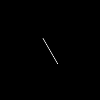
\includegraphics[width=\textwidth]{linear-psf-arr}
		\caption{импульсная характеристика}
		\label{fig:linearPsfArr}
	\end{subfigure}%
	\hfill
	\begin{subfigure}[b]{0.45\textwidth}
		
\includegraphics[width=\textwidth]{linear-psf-fourier}%width=\linewidth
		\caption{амплитудно-частотная характеристика}
		\label{fig:linearPsfFourier}
	\end{subfigure}%
	\caption{Смаз величиной в 30 пикселей под углом $300^{\circ}$}\label{fig:linearPsf}
\end{figure}

\section{Методы восстановления изображения}
Так как в процессе искажения основная операция~--- свёртка, то процессы восстановления изображения основанные на обращении данной операции называются \textit{деконволюцией}. Методы деконволюции разделяются на два класса: итерационные и неитерационные.

Для сравнения исходного и восстановленного изображений $I_1, I_2$ будем использовать две метрики, среднеквадратичную ошибку(СКО) или MSE(mean square error) и пиковое отношение сигнала к шуму PSNR(peak signal to noise ratio) в дБ, которое определим через MSE: 
\begin{equation}\label{eq:mse}
MSE = \frac{1}{MN}\sum_{i=0}^{M-1}\sum_{j=0}^{N-1}\left| I_1(i,j)-I_2(i,j)\right|^2
\end{equation}
\begin{equation}\label{eq:psnr}
PSNR = 20\log_{10}\left(\frac{MAX_I}{\sqrt{MSE}}\right), \text{дБ},
\end{equation}
где $MAX_I$~--- максимальная яркость исходного изображения.

Перед восстановлением, для избежания дребезга края искажённых изображений размываются функцией \verb|edgetaper|.

\subsection{Инверсная фильтрация}
\textit{Инверсная фильтрация}~--- простейший метод восстановления, исходя из модели искажения представленной в частотной области (\ref{eq:distortionFourier}) предполагает следующую оценку спектра восстановленного изображения $\hat{F}(u,v)$~\cite[стр.~411]{gonsalesDigital2012}:
\begin{equation}\label{eq:inverseFiltrationFourier}
\hat{F}(u,v) = \frac{G(u,v)}{H(u,v)}.
\end{equation}
Из (\ref{eq:distortionFourier}) и (\ref{eq:inverseFiltrationFourier}) следует, что
\begin{equation}\label{eq:inverseFiltration}
\hat{F}(u,v) = F(u,v) + \frac{N(u,v)}{H(u,v)}
\end{equation}

Инверсная фильтрация не пригодна для восстановления зашумленных изображений: на частотах, где спектр искажающего оператора близок к нулю второе слагаемое (\ref{eq:inverseFiltration}) вносит очень большой вклад в сумму и как следствие искажает ещё больше оценку исходного изображение.
\begin{figure}[h!]
	\begin{subfigure}[b]{0.5\textwidth}
		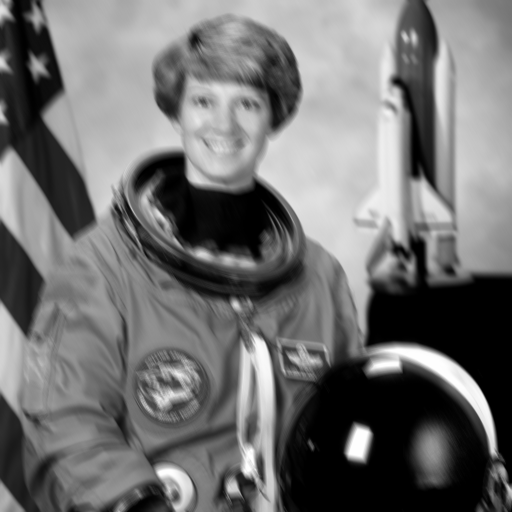
\includegraphics[width=\linewidth]{deconv-astro-shift15}
		\caption{искажённое изображение~--- сдвиг \\на 15 пикселей, шум $\sigma=10^{-5}$}
		\label{fig:astroShift15}
	\end{subfigure}%
	\begin{subfigure}[b]{0.5\textwidth}
		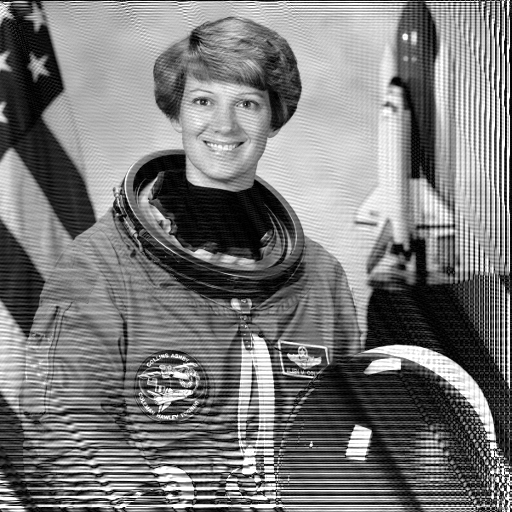
\includegraphics[width=\linewidth]{deconv-inverse-filter}
		\caption{восстановленное изображение\\ PSNR=17.93дБ}
		\label{fig:astroInverseRestored}
	\end{subfigure}%
	\caption{Восстановление изображения размером $512\times 512$ c помощью инверсной фильтрации. Параметры искажения: смаз~--- 15 пикселей, угол $300^\circ$, шум~--- $\sigma_\eta=10^{-5}$}
\end{figure}

При этом шума в камере избежать невозможно: как бы ни была дорога аппаратура, от теплового шума не избавиться.

\subsection{Фильтр Винера}
Основной недостаток инверсной фильтрации~--- неспособность корректно восстанавливать зашумлённые изображения. Чтобы бороться с ним был разработан, в частности, метод \textit{винеровской фильтрации}, использующий свойства функции рассеяния. Основная идея этого алгоритма деконволюции заключается в следующем: изображение и шум рассматриваются как случайные процессы. Ставится следующая задача: необходимо найти такую оценку $\hat{f}$ для исходного изображения $f$, чтобы среднеквадратичное отклонение $e$ этих величин друг от друга было минимальным.

Выполнение этих условий на практике сходится к следующей формуле:
\begin{equation}\label{eq:wiener}
\hat{F}(u,v)=\left(\frac{1}{H(u,v)}\frac{|H(u,v)|^2}{|H(u,v)|^2+K}\right)G(u,v),
\end{equation}
где $K$~--- эмпирически определяемая константа, выбирается так, чтобы получить наилучшее качество восстановления.

\begin{figure}[h!]
	\begin{subfigure}[b]{0.5\textwidth}
		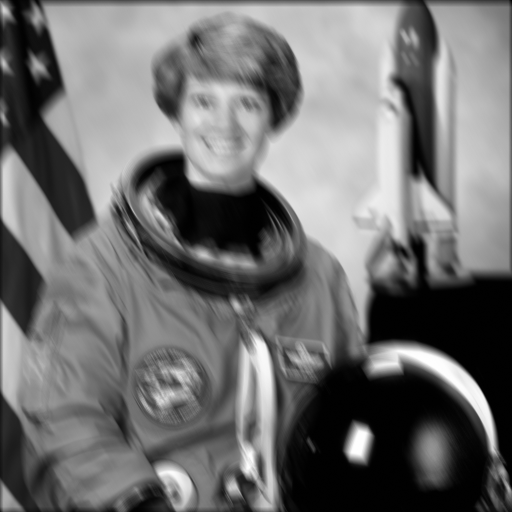
\includegraphics[width=\linewidth]{deconv-shift15}
		\caption{искажённое изображение~--- сдвиг \\на 15 пикселей}
		\label{fig:astroShift15u}
	\end{subfigure}%
	\begin{subfigure}[b]{0.5\textwidth}
		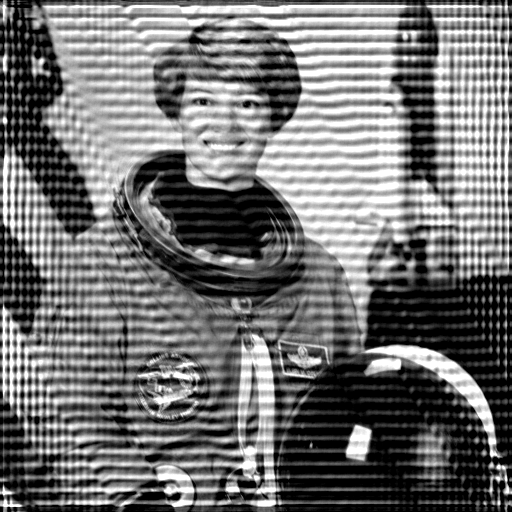
\includegraphics[width=\linewidth]{deconv-shift15-restored-u-wiener}
		\caption{восстановленное изображение\\ PSNR=23.02дБ}
		\label{fig:astroWienerRestored}
	\end{subfigure}%
	\caption{Восстановление изображения размером $512\times 512$ c помощью винеровской фильтрации. Параметры искажения: смаз~--- 15 пикселей, угол $300^\circ$, шум~--- $\sigma_\eta=10^{-3}$}
\end{figure}

На практике не всегда получается получить удовлетворительный результат с помощью выражения (\ref{eq:wiener}). Это происходит из-за того что значения спектров шума и сигнала не известны, а оценка K может быть ошибочна. Кроме того не всегда возможно подбирать этот параметр вручную.

\subsection{Регуляризация по Тихонову}
Существуют методы, для использования которых достаточно знать только среднее значение шума и его дисперсию. Один из таких методов~--- \textit{регуляризация по Тихонову}. Этот метод в спектральной области описывается соотношением~\cite[стр.~418]{gonsalesDigital2012}:
\begin{equation}\label{eq:tikhonov}
\hat{F}(u,v) = \left(\frac{H^*(u,v)}{|H(u,v)|^2 + \gamma|P(u,v)|^2}\right)G(u,v)
\end{equation}

В этом методе от выбора параметра регуляризации $\gamma$ (его выбирают эмпирически или итеративно) зависит качество восстановленного изображения. $P(u,v)$~--- двумерное ДПФ дискретного аналога оператора Лапласа $\nabla^2 = \left(\frac{\partial^2}{\partial x^2} + \frac{\partial^2}{\partial y^2}\right)$:
\begin{equation}
p(x,y) = \begin{bmatrix}
		0 & 1 & 0\\
		1 &-4 & 1\\
		0 & 1 & 0
	\end{bmatrix}
\end{equation}

При $\gamma = 0$ метод вырождается в инверсную фильтрацию. Пример работы алгоритма представлен на рисунке~\ref{fig:tikhonov}
\begin{figure}[h!]
	\begin{subfigure}[b]{0.5\textwidth}
		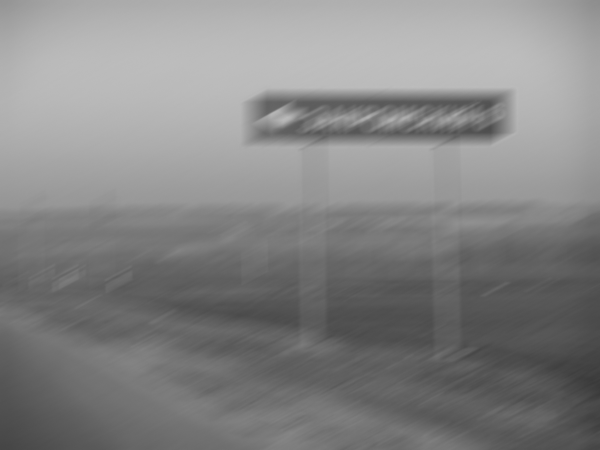
\includegraphics[width=\linewidth]{zakromsky-shift20}
		\caption{искажённое изображение~--- сдвиг \\на 20 пикселей}
		\label{fig:zakromskiyShift20}
	\end{subfigure}%
	\begin{subfigure}[b]{0.5\textwidth}
		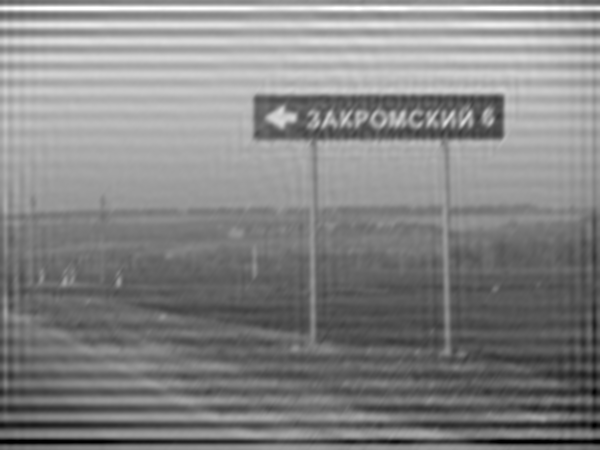
\includegraphics[width=\linewidth]{zakromsky-shift20-tikhonov}
		\caption{восстановленное изображение\\ PSNR=45дБ}
		\label{fig:zakromskiyShift20Tikhonov}
	\end{subfigure}%
	\caption{Восстановление изображения размером $450\times 600$ c помощью регуляризации по Тихонову. Параметры искажения: смаз~--- 20 пикселей, угол $56^\circ$, шум~--- $\sigma_\eta=0.003$}
	\label{fig:tikhonov}
\end{figure}

\subsection{Метод Люси-Ричардсона}
Выше были приведены неитерационные методы. Их недостатком является то, что результат работы сильно зависит от точности определения ИХ $h(x,y)$. Поэтому всё чаще применяются итерационные методы восстановления, которые в процессе работы уточняют ИХ, хотя и требуют больших вычислительных ресурсов. Один из таких методов был предложен независимо друг от друга Л.~Б.~Люси(1974)~\cite{lucy} и В.~Х.~Ричардсоном (1972)~\cite{richardson}. Этот подход основан на использовании метода максимального правдоподобия для изображения, моделируемого в виде статистик Пуассона. Формула для оценки неискажённого изображения $\hat{f}_{k+1}(x,y)$ на $(k + 1)$-ой итерации в \textit{методе Люси-Ричардсона} выглядит следующим образом:
\begin{equation}\label{eq:lucy}
	\hat{f}_{k+1}(x,y) = \hat{f}_k(x,y) \left(h(-x,-y) \conv \frac{g(x,y)}{h(x,y) \conv \hat{f}_k(x,y)}\right)
\end{equation}

Позже были предложены модификации метода Люси-Ричардсона~\cite{richardsonLucyModifiedBiggs}, направленные на увеличение его скорости сходимости и качества восстановленного изображения. В данной работе применяется метод Люси-Ричардсона с модификациями (\ref{eq:lucyMod1} и \ref{eq:lucyMod2}).
\begin{equation}\label{eq:lucyMod1}
	\hat{f}_k=u_k+\alpha_k h_k,
\end{equation}
где $h_k = u_k - u_{k-1}$, $u_k = \hat{f}_k + g_k$, $g_k = \phi(\hat{f}_k)-\hat{f}_k$, $\phi(\hat{f}_k)$~--- результат $(k+1)$-ой итерации алгоритма Люси-Ричардсона~(\ref{eq:lucy}). Эта модификация призвана ускорить работу метода, используя экстраполяцию оценки изображения.   
\begin{equation}\label{eq:lucyMod2}
	\hat{f}_k=\hat{f}_k \cdot C,
\end{equation}
где $C$ — модифицированное ядро Люси-Ричардсона. Ядро $C$ находится следующим образом:
\begin{equation}
	C = p(x,y)^{\gamma-1}\cdot (\gamma-(\gamma-1)p(x,y)),
\end{equation}
где
\begin{equation}
	p(x,y) = \min\left[
		-\frac{2}{t^2}\left(
			g(x,y)\ln\frac{g(x,y)}{J(x,y)}-J(x,y)+g(x,y)
		\right), 1
	\right],
\end{equation}
а $t$~--- пороговое значение, которое определяет уровень затухания(обычно выбирают $t=\sigma/10$, где $\sigma$~--- СКО шума участвующего в искажении исходного изображения), $J(x,y) =h(x,y) \conv \hat{f}_k(x,y)$~--- оценка искажённого изображения. Из эмпирических соображений обычно выбирают $\gamma=10$. Данная модификация повышает точность и сходимость метода. 

\begin{figure}[h!]
	\begin{subfigure}[b]{0.45\textwidth}
		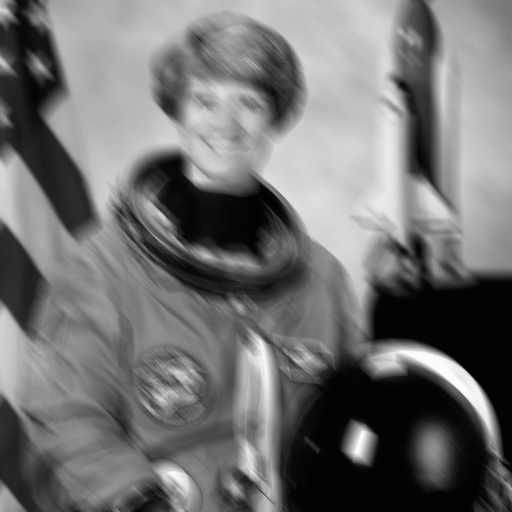
\includegraphics[width=\linewidth]{richardson-lucy-astro-distorted}
		\caption{искажённое изображение~--- сдвиг \\на 20 пикселей}
		\label{fig:astroLucyBlurred}
	\end{subfigure}%
	\hfill
	\begin{subfigure}[b]{0.45\textwidth}
		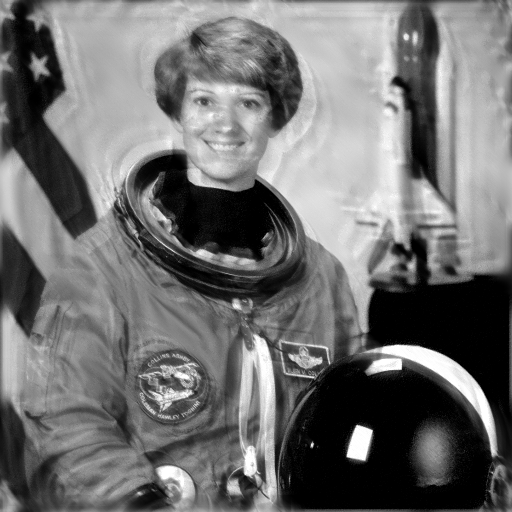
\includegraphics[width=\linewidth]{richardson-lucy-astro-distorted-restored}
		\caption{восстановленное изображение\\ PSNR=21.77дБ}
		\label{fig:astroLucyRestored}
	\end{subfigure}%
	\caption{Восстановление изображения размером $512\times 512$ c помощью метода Люси-Ричардсона. Параметры искажения: смаз~--- 20 пикселей, угол $45^\circ$, шум~--- $\sigma_\eta=0.003$}
	\label{fig:richardsonLucy}
\end{figure}

На рисунке~\ref{fig:richardsonLucy} показан пример работы модифицированного метода Люси-Ричардсона. Как видим, результат работы итерационного метода по качеству превосходит результаты неитерационных методов.


\begin{comment}
%%% не работает без известнй ИХ 
\subsection{Слепая деконволюция}
\end{comment}

\section{Постановка задачи оценки искажающего оператора}
Были рассмотрены несколько методов восстановления изображения. Все они для работы требуют предварительно получить значение ИХ искажающего оператора. Однако в реальных задачах оператор обычно неизвестен и не всегда может быть оценён из параметров сцены. Следовательно необходимо  <<уметь>> получать оценку ИХ из искажённого изображения. Так как метод Люси-Ричардсона на использованных изображениях показал себя лучше других методов, в дальнейшем для процесса деконволюции будем рассматривать только его, а усилия сконцентрируем на создании метода оценки искажающего оператора.
\begin{definition}\label{def:bestPsfEstimaton}
	Наилучшей оценкой $h^*$ искажающего оператора $h$ назовём такую, при использовании которой MSE восстановленного изображения $\hat{f}$ будет минимальна.
	\begin{equation}\label{eq:bestPsf}
	\hat{h}^* = \argmin_{\hat{h}}MSE(f, \hat{f}(g,\hat{h})),
	\end{equation}
\end{definition}
где $\hat{f}(g,h)$~--- оценка восстановленного изображения полученная применением модифицированного метода Люси-Ричардсона к искажённому изображению с оценкой искажающего оператора~$\hat{h}$. 


\chapter{Оценка линейного искажающего оператора}


\chapter{Результаты экспериментов}


\conclusion

Подводим заключение всей нашей эпопее по написанию ВКР.

Также в данном пункте можно вставить благодарности людям, помогавшим в написании работы: маме, дяде Феде с соседнего подъезда и коту.

\bibliographystyle{gost2008}
\bibliography{biblio}

\end{document}

%А в работе \cite{Allen} утверждалось ..., что является противоречием к работе \cite{ARIMA}

% пример цитирования
%В работе \cite{ARIMA} было сказано ...
